\section[Dependability in OpenStack \texorpdfstring{{\textbf{\tiny \enspace (JE, NK)}}}{}]{Dependability in OpenStack}
\sectionmark{Dependability in OpenStack}
\label{dependability}
The dependability aspect of a system is very important when it comes to cloud computing. As cloud computing platforms are usually used to offer infrastructure as a service, even short outages can quickly become expensive. As cloud computing platforms like OpenStack rely on a distributed installation when used in productive mode, it must be ensured that there is no single point of failure, e.g., one node that can bring the whole system down upon failing. This can be accomplished by various means of fault tolerance approaches.\\

In this chapter we will give a basic overview of the analysis of dependability of computing systems based on \cite{Laprie:1992:DBC:573776}, which aims to provide exact definitions of factors that influence the dependability of computer systems. These theoretical foundations are then applied to OpenStack in Chapter~\ref{experiments}.

\subsection{The Term Dependability and Foundations}
The term ``dependability'' is an umbrella term with various, similar definitions. Dependability as defined by \cite{laprie} is 
\begin{quote}
the ability to deliver service that can justifiably be trusted.
\end{quote}
The IFIP working group 10.4\footnote{\url{http://dependability.org/wg10.4/}} defines dependability similarly as
\begin{quote}
the trustworthiness of a computing system which allows reliance to be justifiably placed on the service it delivers.
\end{quote}
Dependability thus adds a third dimension to the evaluation of a system's quality, among cost and performance. This means that a dependable system is one that deals with unexpected events in such a way that its service is not disrupted in a way that the specification is not met. \cite{laprie} further define the elements of dependability in a dependability tree (see Figure~\ref{fig:dependability_tree}).\\

\begin{figure}[h]
	\centering
		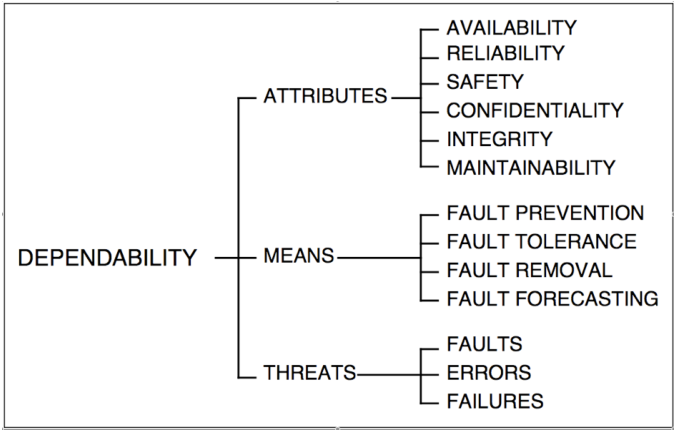
\includegraphics[width=0.60\textwidth]{images/dependability_tree.PNG}
	\caption{Dependability tree as defined by Laprie}
	\label{fig:dependability_tree}
\end{figure}

The attributes are the quality measures of a system. In this masters project, we will mainly analyze the availability and reliability attributes of OpenStack. Reliability is a measure for the continuity of a service, while availability measures the readiness for usage.\\

The dependability threats are system failures, system errors and system faults. A fault is the cause of an error, which is the system state that can then lead to a failure. The failure itself is an event that occurs when the service deviates from the specification. As a result, dependability threats can be seen as a chain, that can iteratively cause further faults, errors and failures through the layers of a system. We will present such dependability threat chains for the experiments we ran on OpenStack in Chapter~\ref{experiments}. \\

The means for handling the dependability threats and thereby improving the dependability attributes are fault prevention, fault tolerance, fault removal and fault forecasting. In fault prevention, the occurrence or introduction of a fault into the system is prevented. A fault tolerant system is able to provide the service as per specification even under faults. Fault removal is reducing the presence of faults in the system, and fault forecasting is estimating the number and consequences of faults. Regarding this masters project, we will look at the first three in relation to OpenStack.

\subsection{Applying Dependability to OpenStack}
When looking at the dependability of very complex systems such as OpenStack it is necessary to decompose the system and consider all layers individually. The bottom most layer we will consider is the infrastructure layer, i.e. the hardware of the nodes on which OpenStack is running and the network connecting them. On top, the OpenStack layer contains all OpenStack services, e.g., networking (Neutron), compute and visualization (Nova) or the identity service (Keystone). The top most layer that we will consider is the application layer, which is the applications on top of the OpenStack layer, e.g., services running on the virtual machines that are deployed on the OpenStack infrastructure. Figure~\ref{fig:depchain} shows an example of a dependability threat chain within the layers of an example OpenStack instance. 

\begin{figure}[h]
	\centering
		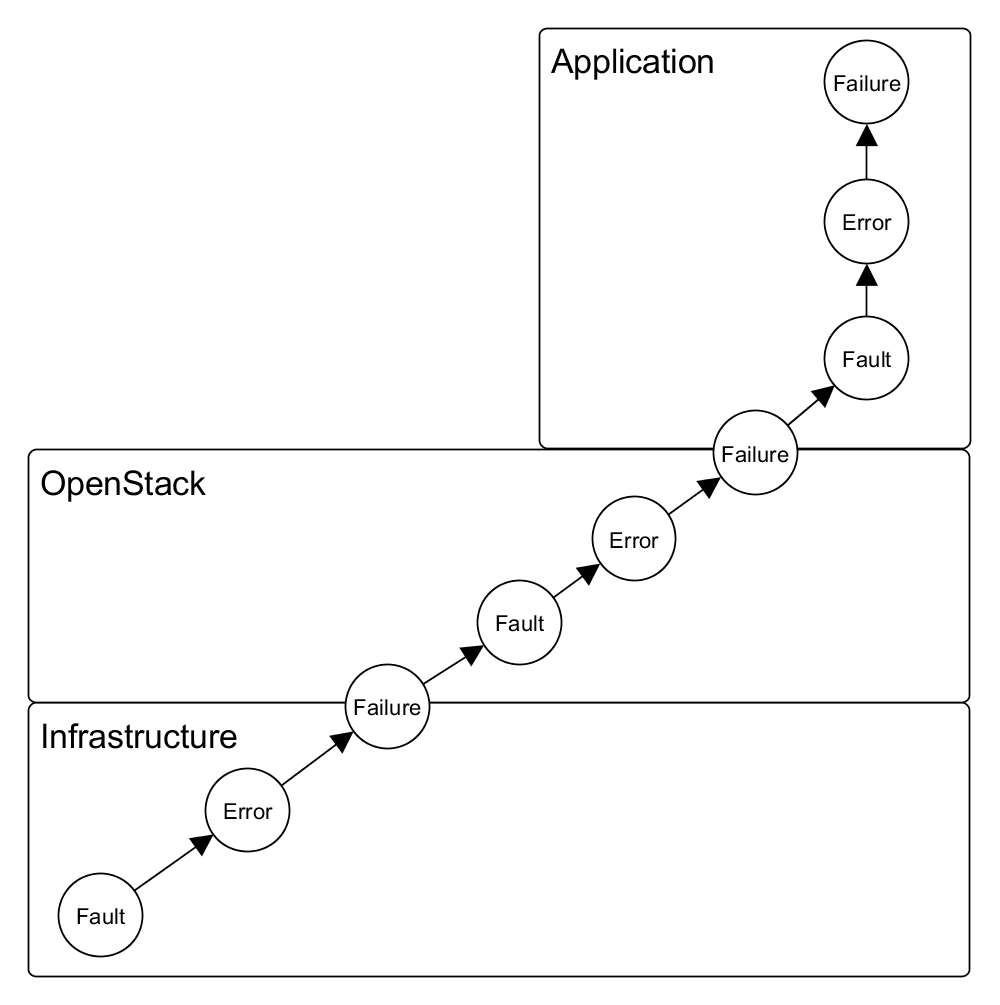
\includegraphics[width=0.60\textwidth]{images/depchain.PNG}
	\caption{Example dependability threat chain through layers of OpenStack}
	\label{fig:depchain}
\end{figure}

As one can see, a fault in a lower layer that leads to a failure can be propagated through the layers until it reaches the application, in which case the user will realize that the application is not running as specified.\\

OpenStack already provides measures of fault tolerance to prevent both system downtime and data loss. These measures are described in the OpenStack high availability guide\footnote{\url{http://docs.openstack.org/high-availability-guide/content/index.html}} for both active/passive and active/active setups. \\

An active/passive setup uses a separate service (such as Pacemaker) to monitor the actual OpenStack services and start passive resources when necessary. For OpenStack, stateless services like Neutron networking or the Glance object storage are suitable for active/passive high availability. \\

An active/active setup has multiple nodes running at the same time with the same services, when one fails over, the rest will take the load. In OpenStack, mainly the stateful services like the RabbitMQ message queue and the MySQL database will require an active/active setup. \\

With these dependability insights we were able to run dependability analysis on our OpenStack test environment. To do so, an OpenStack failure has to be specified. We define a failure of the OpenStack system with regard to the use case of downloading, uploading or streaming files from a virtual machine of a user. We then define a list of faults, that can cause the defined failure, and categorized them into virtual machine faults (server on VM not reachable, no network for VM, etc.), network faults (broken networking hardware, etc.), storage faults (broken hard drives, etc.) and OpenStack faults (Keystone crash, swift crash, etc.). The results of the experiments that test the dependability on the test environment will be described in Chapter~\ref{experiments}.\\

To conclude, with our master project system we are able to inject faults into our test environment and thus evaluate the fault tolerance of the OpenStack system. If the system thereby behaves in an unspecified manner, one is able to find possible bugs in OpenStack and if possible, one might be able to fix them, achieving a fault prevention this way. Over all, we draw insights about the reliability of OpenStack in relation to the test environment used in Chapter~\ref{experiments}.\\


